\documentclass{beamer}

\title{How to (not) Store Your Passwords}
\subtitle{\url{https://github.com/rlindsgaard/presentations/tree/master/2017-03-18-how-to-not-store-your-passwords}}
\author{Ronni Elken Lindsgaard \\ rel@zx.dk \\ @rlindsgaard}
\date{2017-03-18}

\usetheme{metropolis}

\usepackage{graphicx}
\usepackage{alltt}

\begin{document}

\begin{frame}
  \maketitle
\end{frame}

\begin{frame}
  \tableofcontents
\end{frame}

\section{Analysis}
\begin{frame}{General Password Security}
  \begin{block}{}
    \begin{itemize}
      \item Don't store in plain-text
      \item Don't re-use passwords
      \item Make secure passwords
    \end{itemize}
  \end{block}
\end{frame}

\begin{frame}{Secure passwords}
  \begin{itemize}
    \item High entropy (e.g. NIST\footnote{\url{http://wayback.archive.org/web/20040712152833/http://csrc.nist.gov/publications/nistpubs/800-63/SP800-63v6_3_3.pdf}})
    \item Passphrases: a sentence that is not too long to remember
    \item Schneier Scheme: ASSt's!2\_2r \footnote{\url{https://www.schneier.com/blog/archives/2014/03/choosing_secure_1.html}, \url{https://www.schneier.com/essays/archives/2008/11/passwords_are_not_br.html}}
    \item Troy Hunt: Should be too complex to remember! \footnote{\url{https://www.troyhunt.com/only-secure-password-is-one-you-cant/}, \url{http://robinmessage.com/2014/03/why-bruce-schneier-is-wrong-about-passwords/}}
  \end{itemize}
\end{frame}

\begin{frame}{Online password managers}
  \footnotesize
  \begin{table}
    \begin{tabular}{c|c|c}
      \textbf{Strengths} & \textbf{Weaknesses} & \textbf{Attack vectors} \\
      \hline
      Portability & Availability & Database compromise \\
      \hline
      Organisational sharing & One key to the kingdom & Meta-data leakage \\
      \hline
      Recoverable & & 3rd party \\
      \hline
      Strong passwords & & Keylogging \\
      \hline
      Known secrets & & \\
    \end{tabular}
  \end{table}
\end{frame}

\begin{frame}{Offline password managers}
  \footnotesize
  \begin{table}
    \begin{tabular}{c|c|c}
      \textbf{Strengths} & \textbf{Weaknesses} & \textbf{Attack vectors} \\
      \hline
      Trusted storage & Backup & Data-loss \\
      \hline
      Strong passwords & User interface & Computer/data compromise \\
      \hline
      No 3rd party & & Keylogging \\
      \hline
      No meta-data & & \\
      \hline
      Known secrets & & \\
    \end{tabular}
  \end{table}
\end{frame}

\begin{frame}{Bottom line}
  \begin{block}{}
    \begin{center}
      Data are susceptible to being either lost or stolen.
    \end{center}
  \end{block}
\end{frame}

\begin{frame}{Let's make things better}
  \begin{itemize}
    \item Secure domain specific passwords
    \item Portable
    \item Configurable to website rules
    \item {\color{red} No storage needed!}
  \end{itemize}
\end{frame}

\section{Methodology}
\subsection{Generating Secure Passwords}
\begin{frame}[fragile]{Deterministic Pseudo Random Number}
  \begin{block}{}
    \begin{verbatim}
    % echo "naturalbornhacker" | md5sum -
    04d1530d764932ccbff01c185a283c8e  -
    \end{verbatim}
  \end{block}
\end{frame}

\begin{frame}[fragile]{Generating the password}
  \begin{block}{}
    \begin{alltt}
hash = {\color{red}0}4d1530d764932ccbff
alphabet = {\color{green}a}bcdABCD1234!"#_

password = a
    \end{alltt}
  \end{block}
\end{frame}

\begin{frame}[fragile]{Generating the password}
  \begin{block}{}
    \begin{alltt}
hash = 0{\color{red}4}d1530d764932ccbff
alphabet = abcd{\color{green}A}BCD1234!"#_

password = aA
    \end{alltt}
  \end{block}
\end{frame}

\begin{frame}[fragile]{Generating the password}
  \begin{block}{}
    \begin{alltt}
hash = 04{\color{red}d}1530d764932ccbff
alphabet = abcdABCD1234!{\color{green}"}#_

password = aA"
    \end{alltt}
  \end{block}
\end{frame}


\begin{frame}[fragile]{Generating the password}
  \begin{block}{}
    \begin{alltt}
hash = 04d1530d764932ccbff
alphabet = abcdABCD1234!"#_

password = aA"bBda"DCA2dc!!__
    \end{alltt}
  \end{block}
\end{frame}

\begin{frame}[fragile]{Domain specific passwords}
  \begin{block}{}
    \begin{verbatim}
function g(str password, str context) {
  echo hash(password + context)
}
g("1234", "opensourcedays.org")
// puK5hbxzwjsE0s#pNO6sR&TcFn4<;x"q
g("1234", "github.com")
// &D8s1zM_rHAe$uuRysn>JO#Rv|oZ%j/d
    \end{verbatim}
  \end{block}
\end{frame}

\begin{frame}[fragile]{Master key}
  \begin{itemize}
    \item Salt
    \item Mitigate shoulder surfing
    \item Partial compromise on typing
  \end{itemize}
\end{frame}

\begin{frame}[fragile]{Master Key use}
  \begin{block}{}
    \begin{verbatim}
function g(str salt, str password, str context) {
  echo hash(salt, password + context)
}
g("correct horse battery staple", "1234",
  "opensourcedays.org")
// L>nZQ]/Xb-Q$^i[cU1h@!4.mt+UGheV,
g("correct horse battery staple", "1234",
  "github.com")
// `mD*u,!.}u'Xklr _hNZCd5!SQ6clFGz
    \end{verbatim}
  \end{block}
\end{frame}

\section{Security discussion}
\subsection{Attack vectors}
\begin{frame}{Attack vectors}
  \begin{itemize}
    \item Keylogging
    \item Shoulder surfing
    \item Brute force
  \end{itemize}
\end{frame}

\begin{frame}{Bruteforcing}
  \begin{itemize}
    \item PwdHash
    \item David Llewellyn-Jones and Graham Rymer
    \item Cracking PwdHash: A Bruteforce Attack on Client-side Password Hashing
  \end{itemize}
\end{frame}

\begin{frame}{Findings}
  \begin{itemize}
    \item TL;DR: Generated password entropy O(password)
    \item Master key (salt) + Group key
    \item Memory heavy hash function (PBKDF2)
  \end{itemize}
\end{frame}

\begin{frame}{Deterministic Manager Analysis}
  \footnotesize
  \begin{table}
    \begin{tabular}{c|c|c}
      \textbf{Strengths} & \textbf{Weaknesses} & \textbf{Attack vectors} \\
      \hline
      Portable & Backups & Keylogging \\
      \hline
      No meta-data & Known secrets & Brute-force \\
      \hline
      No 3rd party & & \\
    \end{tabular}
  \end{table}
\end{frame}

\section{Introducing RndPhrase Improved}

\begin{frame}{User interface example}
  \begin{center}
    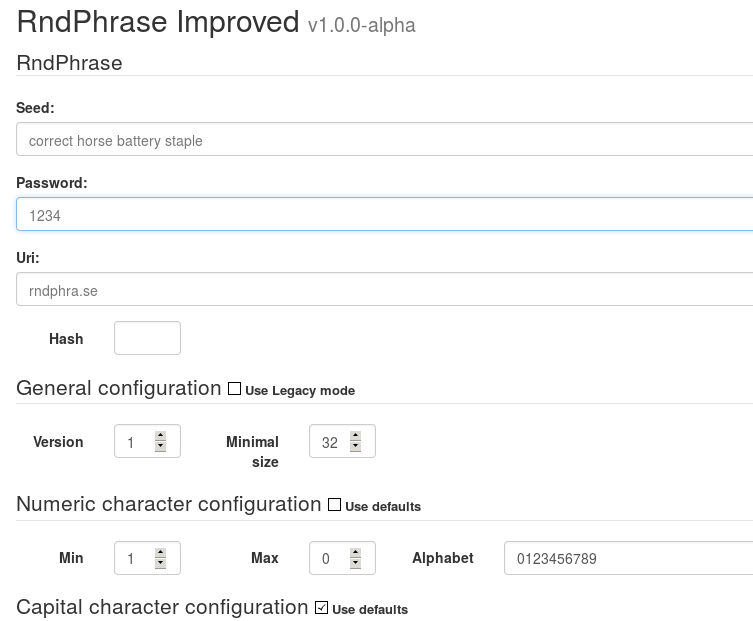
\includegraphics[scale=0.35]{rndphrase-screenshot.png}
  \end{center}
\end{frame}

\begin{frame}{Introducing RndPhrase Improved}
  \begin{itemize}
    \item 1.0.0-alpha2
    \item PBKDF2 for hashing (WebCrypto)
    \item Configurable alphabet
    \item Character occurence constraints
    \item Configurable size
    \item Re-use credentials (versions)
  \end{itemize}
\end{frame}

\begin{frame}{Roadmap}
  \begin{block}{Beta}
    \begin{itemize}
      \item At least 1 more peer review
      \item WebExtensions plugin
    \end{itemize}
  \end{block}
  \begin{block}{Stable}
    \begin{itemize}
      \item Waiting for Candidate Recommendations: WebCrypto, Encoding
    \end{itemize}
  \end{block}
\end{frame}

\begin{frame}{Would You Like To Learn More?}
  \begin{itemize}
    \item \url{https://rndphra.se}
    \item \url{https://github.com/RndPhrase}
    \item \url{http://rlindsgaard.github.io/2016/01/29/rndphrase-roadmap.html}
  \end{itemize}
\end{frame}
\section*{Bonus Slides}
\begin{frame}{Another Piece to the Puzzle}
  \begin{block}{}
   \end{block}{}
\end{frame}

\begin{frame}{}
  \begin{block}{Questions?}
  \end{block}
\end{frame}

\end{document}
